\section{Proposta de solução}

\begin{frame}{Proposta de solução}

    \begin{figure}[h]
        \centering
        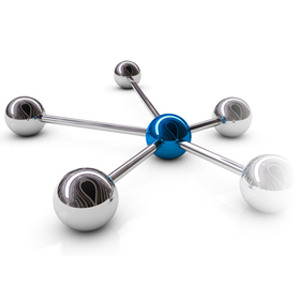
\includegraphics[scale=.8]{images/small-graph}
    \end{figure}
\end{frame}

\begin{frame}{Proposta de solução}
    
    \begin{itemize}
        \setlength{\itemsep}{.5cm}
        \item Uma abstração da rede em forma de um módulo em grafos 
        \item Esse grafo, em tempo real, é a base para computações na rede
        \item A solução objetiva simplificar a análise e o gerenciamento 
            em redes
    \end{itemize}

\end{frame}

\begin{frame}{Modelagem do grafo}

    \begin{itemize}
        \setlength{\itemsep}{.5cm}
        \item $G=(V, A)$, em que $V$ e $A$ são conjuntos finitos de vértices 
            e arestas, respectivamente.
        \item Cada vértice $v \in V$ é um computador ou \emph{switch}.
        \item Cada aresta $u \to v \in A$ é um enlace entre dois vértices.
        \item O peso das arestas $g(u, v)$ é quantidade de \emph{bytes} 
            trafegados na aresta entre os dois vértices.
    \end{itemize}
\end{frame}

\begin{frame}{Classes}

    \begin{columns}[T] % align columns
        \begin{column}{.33\textwidth}

            \begin{itemize}
                \setlength{\itemsep}{.5cm}
                \item{Graph}
                \item{GraphEntity}
                \item{Vertex}
                \item{Edges} 
                \item{GraphManager}
            \end{itemize}
        \end{column}%
        \hfill%
        \begin{column}{.67\textwidth}
            \begin{figure}[h]
                \centering
                
\includegraphics[scale=.4]{images/graph-interfaces}
            \end{figure}
        \end{column}%
    \end{columns}

\end{frame}

\begin{frame}{Interface de programação}

    \begin{columns}[T] % align columns
        \begin{column}{.33\textwidth}

            \begin{itemize}
                \setlength{\itemsep}{.5cm}
                \item \emph{get\_vertex(id)}
                \item \emph{get\_adjacents(id)}
                \item \emph{snapshot()}
                \item \emph{get\_mst()}
            \end{itemize}
        \end{column}%
        \hfill%
        \begin{column}{.67\textwidth}
            \begin{figure}[h]
                \centering
                
\includegraphics[scale=4]{images/gear}
            \end{figure}
        \end{column}%
    \end{columns}

\end{frame}

\begin{frame}{Integração entre módulos}

\begin{figure}[h!]
    \centering
    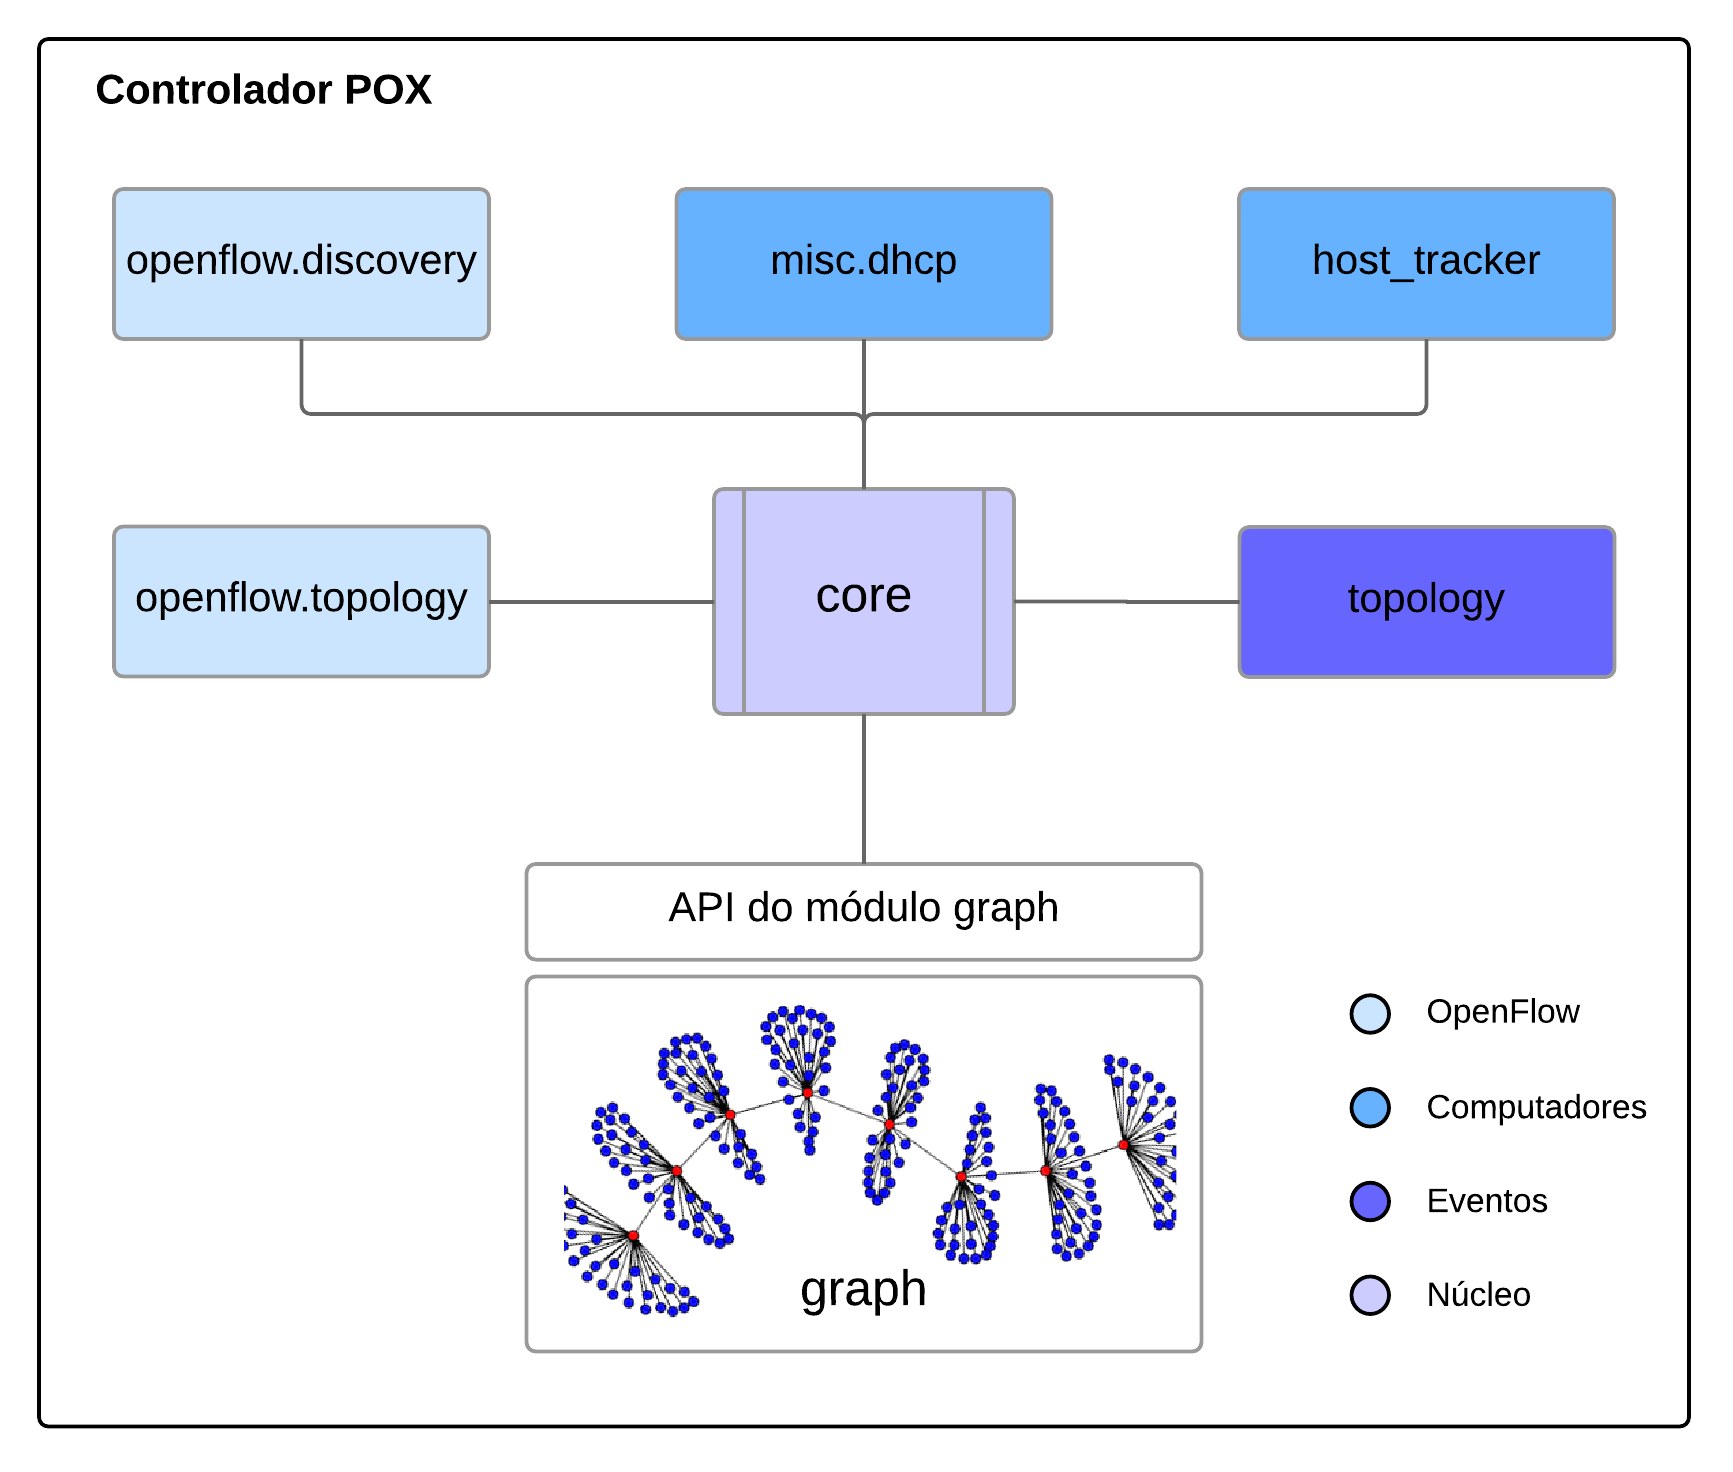
\includegraphics[scale=.55]{images/graph-module-integration}
\end{figure}

\end{frame}
